\documentclass[MASTER.tex]{subfiles} 
\begin{document} 
\begin{frame}
\begin{figure}
\centering
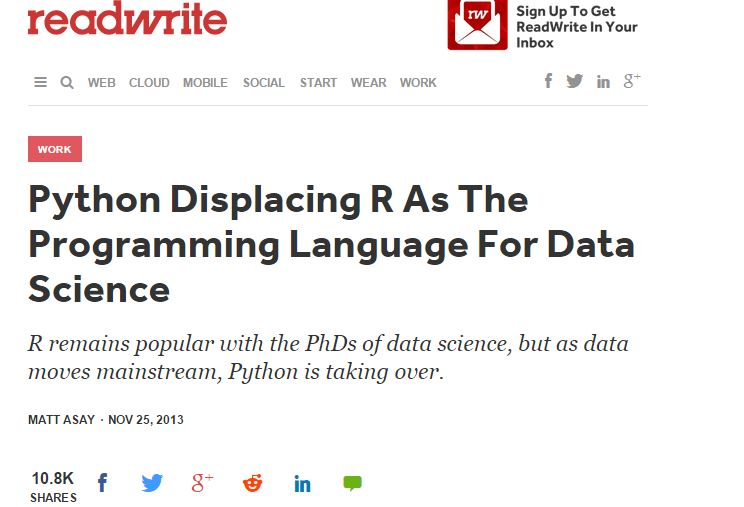
\includegraphics[width=1.05\linewidth]{mjasay}

\end{figure}

\end{frame}
	%----------------------------------------------------------------------------------------------------%
		\begin{frame}
		\begin{figure}
\centering

\includegraphics[width=1.05\linewidth]{pydatalogo}

\end{figure}

	\end{frame}
%===========================================================%
\begin{frame}
	\frametitle{PyData :  Conference Mission}
	\large
	
	\begin{itemize}
	\item PyData is a gathering of users and developers of data analysis tools in Python. \bigskip
	\item The goals are to provide Python enthusiasts a place to share ideas and learn from each other about how best to apply our language and tools to ever-evolving challenges in the vast realm of data management, processing, analytics, and visualization.
	\end{itemize}

	
\end{frame}
%===========================================================%
\begin{frame}
	\large
	\frametitle{PyData}
	\large
	\begin{itemize}
		\item We aim to be an accessible, community-driven conference, with tutorials for novices, advanced topical workshops for practitioners, and opportunities for package developers and users to meet in person.
		
		\item A major goal of the conference is to provide a venue for users across all the various domains of data analysis to share their experiences and their techniques, as well as highlight the triumphs and potential pitfalls of using Python for certain kinds of problems.
	\end{itemize}
\end{frame}
%===========================================================%
%=========================================================== %
\begin{frame}
\begin{figure}
\centering

\includegraphics[width=1.0\linewidth]{continuum}
\end{figure}
	\end{frame}
	%=========================================================== %
	\begin{frame}\begin{figure}
\centering

\includegraphics[width=1.05\linewidth]{pydataberlin}

\end{figure}
	\end{frame}
	%=========================================================== %
	\begin{frame}
		\begin{figure}

\centering
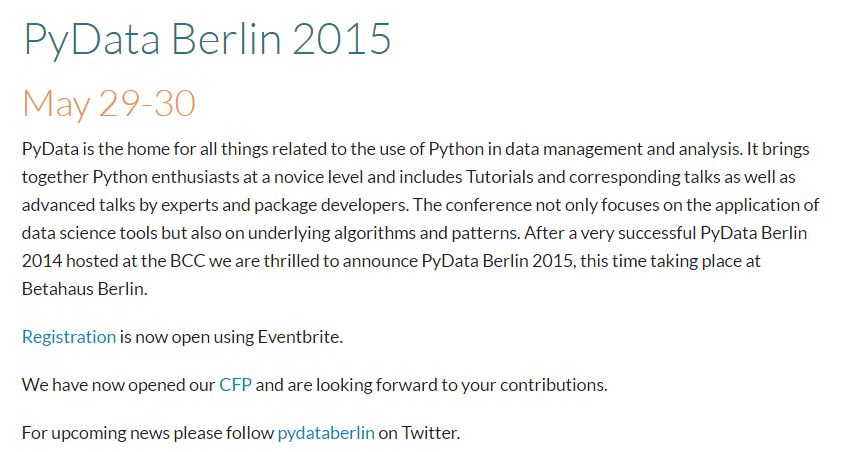
\includegraphics[width=1.10\linewidth]{pydataberlinsiteinfo}

\end{figure}
\end{frame}
%================================================================== %
\begin{frame}
	
\begin{figure}
\centering
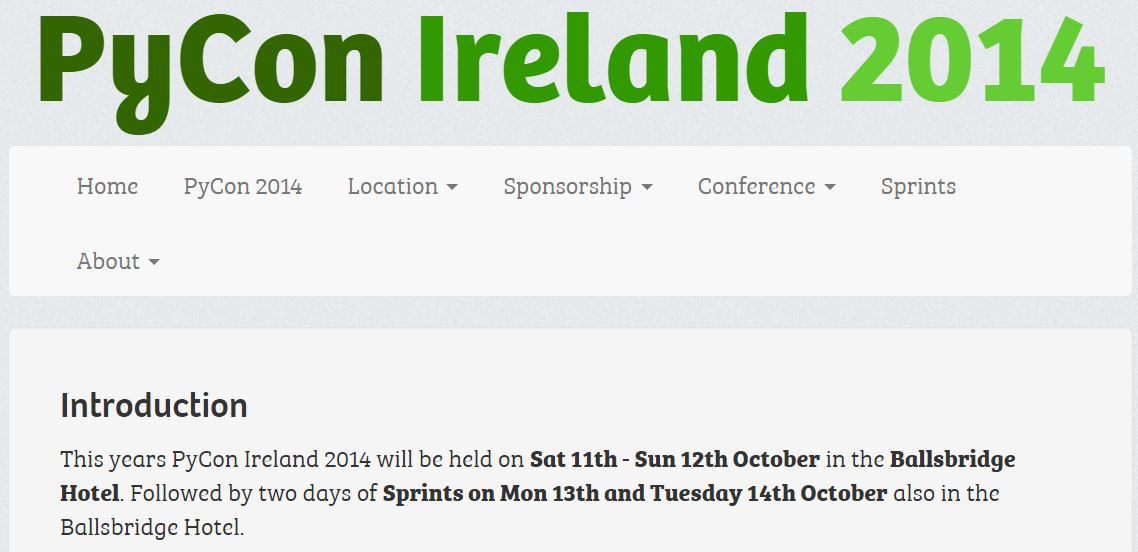
\includegraphics[width=1.1\linewidth]{pyconsiteinfo}

\end{figure}
\end{frame}
%================================================================== %
\begin{frame}
\begin{figure}
\centering
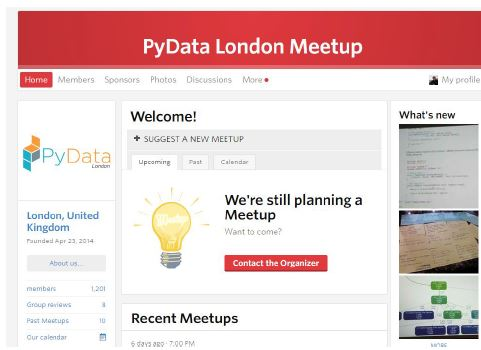
\includegraphics[width=1.1\linewidth]{pydatalondon}
\end{figure}
\end{frame}
%================================================================== %


\end{document}